\documentclass[12pt,a4paper]{article}

% ── Packages ───────────────────────────────────────────────────────────────
\usepackage[margin=2.5cm, headheight=15pt]{geometry}
\usepackage{graphicx}
\usepackage{pdfpages}
\usepackage{comment}
\usepackage{hyperref}
\usepackage{listings}
\usepackage{xcolor}
\usepackage{tikz}
\usetikzlibrary{shapes.geometric, arrows.meta, positioning, fit, backgrounds, decorations.pathreplacing}
\usepackage{booktabs}
\usepackage{multirow}
\usepackage{caption}
\usepackage{parskip}
\usepackage{titlesec}
\usepackage{fancyhdr}
\usepackage{amsmath}

% ── Page style ─────────────────────────────────────────────────────────────
\pagestyle{fancy}
\fancyhf{}
\rhead{Assignment 1}
\lhead{ECE F343: Communication Networks}
\cfoot{\thepage}

% ── Listing style (C code) ─────────────────────────────────────────────────
\definecolor{codebg}{RGB}{245,245,245}
\definecolor{keywordcolor}{RGB}{0,0,200}
\definecolor{commentcolor}{RGB}{60,130,60}
\definecolor{stringcolor}{RGB}{180,0,0}

\lstdefinestyle{cstyle}{
    language=C,
    backgroundcolor=\color{codebg},
    basicstyle=\ttfamily\small,
    keywordstyle=\color{keywordcolor}\bfseries,
    commentstyle=\color{commentcolor}\itshape,
    stringstyle=\color{stringcolor},
    numberstyle=\tiny\color{gray},
    numbers=left,
    stepnumber=1,
    numbersep=8pt,
    frame=single,
    framerule=0.4pt,
    breaklines=true,
    breakatwhitespace=false,
    tabsize=4,
    showstringspaces=false,
    captionpos=b,
}

% ── TikZ styles ────────────────────────────────────────────────────────────
\tikzset{
    layer/.style={
        rectangle, rounded corners=4pt,
        minimum width=8.5cm, minimum height=0.9cm,
        text centered, draw=black, thick,
        font=\sffamily\small
    },
    app/.style    ={layer, fill=blue!20},
    pres/.style   ={layer, fill=cyan!20},
    sess/.style   ={layer, fill=teal!20},
    tran/.style   ={layer, fill=green!25},
    net/.style    ={layer, fill=yellow!30},
    dl/.style     ={layer, fill=orange!30},
    phy/.style    ={layer, fill=red!20},
    arrow/.style  ={-{Stealth[length=6pt]}, thick},
    hdrlabel/.style={font=\ttfamily\tiny, text=gray, right=0.15cm}
}

\title{ECE F343: Communication Networks \\ \Large{Assignment 1}}
\author{Pranav Chandra N. V. \\ 2023AAPS0013P}
\date{26/06/2026}
% ── Document ───────────────────────────────────────────────────────────────
\begin{document}
\maketitle
\tableofcontents
\newpage

\section*{Notes}
All files and additional source files may be found on the associated \href{https://github.com/Prachannagven/commnet-assignment-1}{GitHub repository}. All programs were written/run on a Ubuntu system.

\section{Quesition 1}
\subsection{Introduction}

This program was written for Assignment 1, Question 1. The goal is to show
how message encapsulation works in the OSI model by simulating the
downward flow of data from Layer 7 (Application) to Layer 1 (Physical).

The user enters a message of up to 80 characters. The program passes it
through seven functions, one per layer. Each function sticks its own header
onto the front of whatever it received, prints the result, and then calls
the function for the layer below it.

\subsection{OSI Reference Model Overview}

The OSI model splits network communication into seven layers, each with a
specific job. Table~\ref{tab:osi} lists each layer, the name for its unit
of data (PDU), and the header string used in this program.

\begin{table}[h!]
	\centering
	\begin{tabular}{clll}
		\toprule
		\textbf{Layer} & \textbf{Name} & \textbf{PDU} & \textbf{Simulated Header}                             \\
		\midrule
		7              & Application   & Message      & \texttt{[APP: HTTP GET /index.html]}                  \\
		6              & Presentation  & Message      & \texttt{[PRES: ENC=UTF-8 FORMAT=ASCII COMPRESS=NONE]} \\
		5              & Session       & Message      & \texttt{[SESS: ID=A1B2C3 SEQ=001 TYPE=DATA]}          \\
		4              & Transport     & Segment      & \texttt{[TRAN: TCP SRC=1234 DST=80 SEQ=100 ACK=0]}    \\
		3              & Network       & Packet       & \texttt{[NET: SRC=192.168.1.1 DST=10.0.0.1 TTL=64]}   \\
		2              & Data Link     & Frame        & \texttt{[DL: SRC=AA:BB:CC DST=11:22:33 TYPE=IPv4]}    \\
		1              & Physical      & Bits         & \texttt{[PHY: ENC=NRZ SIGNAL=DIGITAL]}                \\
		\bottomrule
	\end{tabular}
	\caption{OSI Layers, PDU names, and simulated headers}
	\label{tab:osi}
\end{table}

\subsection{Design Decisions}

\begin{itemize}
	\item A helper function \texttt{prepend\_header()} takes care of copying
	      the header and message into a new buffer, so the layer functions
	      themselves stay short and readable.
	\item Buffers are fixed-size arrays on the stack (\texttt{MAX\_BUF = 1024}
	      bytes). This is more than enough for seven headers plus an 80-char
	      message, and the helper exits if that ever overflows.
	\item All headers are kept under 64 characters as required by the spec.
	\item Each layer function just calls the one below it directly, keeping
	      the call chain simple and easy to follow.
\end{itemize}

\newpage
\subsection{Constants and Macros}

\begin{lstlisting}[style=cstyle, caption={Buffer and header constants}]
#define MAX_APP_MSG  80    
#define MAX_HEADER   64   
#define MAX_BUF      1024

#define HDR_APP   "[APP: HTTP GET /index.html]"
#define HDR_PRES  "[PRES: ENC=UTF-8 FORMAT=ASCII COMPRESS=NONE]"
#define HDR_SESS  "[SESS: ID=A1B2C3 SEQ=001 TYPE=DATA]"
#define HDR_TRAN  "[TRAN: TCP SRC=1234 DST=80 SEQ=100 ACK=0]"
#define HDR_NET   "[NET: SRC=192.168.1.1 DST=10.0.0.1 TTL=64]"
#define HDR_DL    "[DL: SRC=AA:BB:CC DST=11:22:33 TYPE=IPv4]"
#define HDR_PHY   "[PHY: ENC=NRZ SIGNAL=DIGITAL]"
\end{lstlisting}

\subsection{Helper: \texttt{prepend\_header()}}

\begin{lstlisting}[style=cstyle, caption={Header prepending helper}]
static int prepend_header(const char *header, const char *msg, int msg_size, char *out_buf, int out_buf_size){
    int hdr_len  = (int)strlen(header);
    int new_size = hdr_len + msg_size;

    if (new_size >= out_buf_size) {
        fprintf(stderr, "Buffer overflow prevented.\n");
        exit(1);
    }

    memcpy(out_buf,           header, hdr_len);
    memcpy(out_buf + hdr_len, msg,    msg_size);
    out_buf[new_size] = '\0';

    return new_size;
}
\end{lstlisting}

\subsection{Layer Functions}

All seven layer functions work the same way:

\begin{enumerate}
	\item Allocate a local buffer (\texttt{MAX\_BUF} bytes).
	\item Call \texttt{prepend\_header()} to build the new PDU.
	\item Print it.
	\item Call the next layer down (the Physical layer skips this last step).
\end{enumerate}

\newpage
\begin{lstlisting}[style=cstyle, caption={Application Layer (representative example)}]
void application_layer(char *msg, int size)
{
    char buf[MAX_BUF];
    int  new_size = prepend_header(HDR_APP, msg, size, buf, MAX_BUF);
    printf("[Layer 7 - Application]  PDU: %s\n\n", buf);
    presentation_layer(buf, new_size);
}
\end{lstlisting}

% ═══════════════════════════════════════════════════════════════════════════
\subsection{Message Flow Flowchart}
% ═══════════════════════════════════════════════════════════════════════════

Figure~\ref{fig:flowchart} shows the message moving down through the layers.
The PDU gets longer at each step as another header is added to the front.

\begin{figure}[h!]
	\centering
	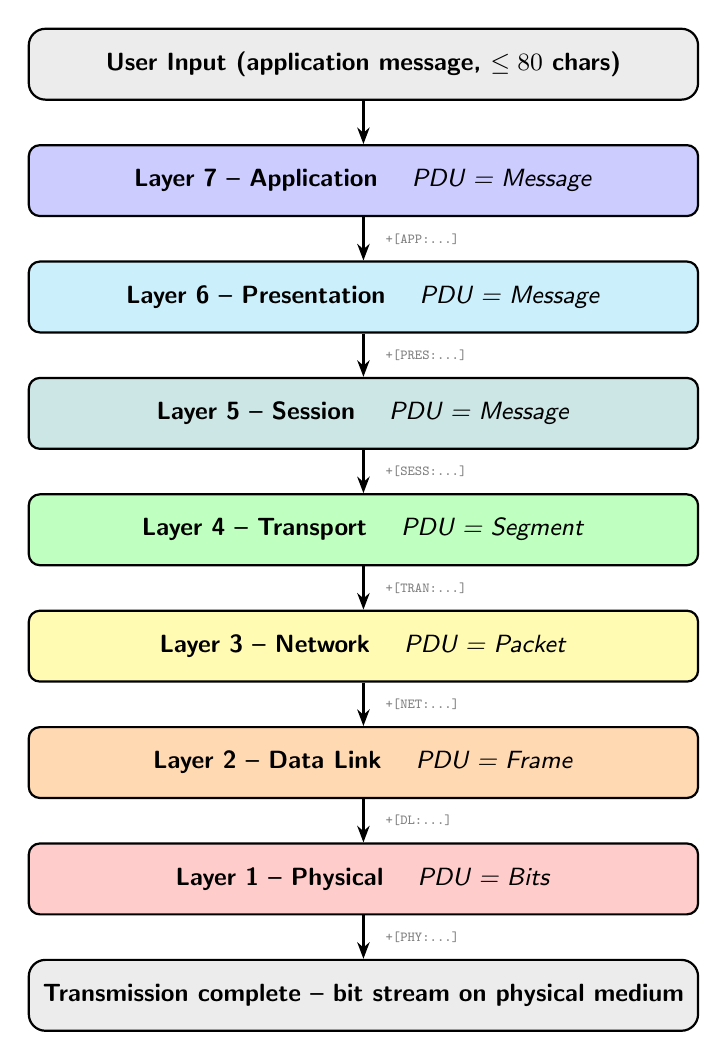
\begin{tikzpicture}[node distance=0.55cm and 2cm]

		% ── Input ──────────────────────────────────────────────────────────────
		\node[rectangle, rounded corners=6pt, draw, fill=gray!15, thick,
			minimum width=8.5cm, minimum height=0.9cm,
			font=\sffamily\small\bfseries] (input)
		{User Input (application message, $\leq 80$ chars)};

		% ── Layers ─────────────────────────────────────────────────────────────
		\node[app,  below=of input]  (L7) {\textbf{Layer 7 -- Application}  \quad\textit{PDU = Message}};
		\node[pres, below=of L7]     (L6) {\textbf{Layer 6 -- Presentation} \quad\textit{PDU = Message}};
		\node[sess, below=of L6]     (L5) {\textbf{Layer 5 -- Session}      \quad\textit{PDU = Message}};
		\node[tran, below=of L5]     (L4) {\textbf{Layer 4 -- Transport}    \quad\textit{PDU = Segment}};
		\node[net,  below=of L4]     (L3) {\textbf{Layer 3 -- Network}      \quad\textit{PDU = Packet}};
		\node[dl,   below=of L3]     (L2) {\textbf{Layer 2 -- Data Link}    \quad\textit{PDU = Frame}};
		\node[phy,  below=of L2]     (L1) {\textbf{Layer 1 -- Physical}     \quad\textit{PDU = Bits}};

		% ── Output ─────────────────────────────────────────────────────────────
		\node[rectangle, rounded corners=6pt, draw, fill=gray!15, thick,
			minimum width=8.5cm, minimum height=0.9cm,
			font=\sffamily\small\bfseries, below=of L1] (output)
		{Transmission complete -- bit stream on physical medium};

		% ── Arrows ─────────────────────────────────────────────────────────────
		\draw[arrow] (input) -- (L7);
		\draw[arrow] (L7)    -- node[hdrlabel] {\texttt{+[APP:...]}} (L6);
		\draw[arrow] (L6)    -- node[hdrlabel] {\texttt{+[PRES:...]}} (L5);
		\draw[arrow] (L5)    -- node[hdrlabel] {\texttt{+[SESS:...]}} (L4);
		\draw[arrow] (L4)    -- node[hdrlabel] {\texttt{+[TRAN:...]}} (L3);
		\draw[arrow] (L3)    -- node[hdrlabel] {\texttt{+[NET:...]}} (L2);
		\draw[arrow] (L2)    -- node[hdrlabel] {\texttt{+[DL:...]}} (L1);
		\draw[arrow] (L1)    -- node[hdrlabel] {\texttt{+[PHY:...]}} (output);
		\begin{comment}

		% ── Encapsulation brace label ───────────────────────────────────────────
		\draw [decorate, decoration={brace, amplitude=6pt}, thick, gray]
		([xshift=4.5cm] L7.north east) -- ([xshift=4.5cm] L1.south east)
		node [midway, right=10pt, font=\sffamily\scriptsize, text=gray,
			align=center] {Each layer\\prepends\\its header};

		\end{comment}

	\end{tikzpicture}
	\caption{Message flow and encapsulation across the OSI 7 layers.}
	\label{fig:flowchart}
\end{figure}

% ═══════════════════════════════════════════════════════════════════════════
\newpage
\subsection{Sample Output}

Running the program with the input \texttt{"Hello, Network!"} gives:

\begin{lstlisting}[style=cstyle, language={}, caption={Sample program output}]
Enter application message (up to 80 characters):
> hello world!

=== OSI Encapsulation ===

[Layer 7 - Application]  PDU:
[APP: HTTP GET /index.html]hello world!

[Layer 6 - Presentation] PDU:
[PRES: ENC=UTF-8 FORMAT=ASCII COMPRESS=NONE][APP: HTTP GET /index.html]hello world!

[Layer 5 - Session]      PDU:
[SESS: ID=A1B2C3 SEQ=001 TYPE=DATA][PRES: ENC=UTF-8 FORMAT=ASCII COMPRESS=NONE][APP: HTTP GET /index.html]hello world!

[Layer 4 - Transport]    Segment:
[TRAN: TCP SRC=1234 DST=80 SEQ=100 ACK=0][SESS: ID=A1B2C3 SEQ=001 TYPE=DATA][PRES: ENC=UTF-8 FORMAT=ASCII COMPRESS=NONE][APP: HTTP GET /index.html]hello world!

[Layer 3 - Network]      Packet:
[NET: SRC=192.168.1.1 DST=10.0.0.1 TTL=64][TRAN: TCP SRC=1234 DST=80 SEQ=100 ACK=0][SESS: ID=A1B2C3 SEQ=001 TYPE=DATA][PRES: ENC=UTF-8 FORMAT=ASCII COMPRESS=NONE][APP: HTTP GET /index.html]hello world!

[Layer 2 - Data Link]    Frame:
[DL: SRC=AA:BB:CC DST=11:22:33 TYPE=IPv4][NET: SRC=192.168.1.1 DST=10.0.0.1 TTL=64][TRAN: TCP SRC=1234 DST=80 SEQ=100 ACK=0][SESS: ID=A1B2C3 SEQ=001 TYPE=DATA][PRES: ENC=UTF-8 FORMAT=ASCII COMPRESS=NONE][APP: HTTP GET /index.html]hello world![FCS: 0xF47B14F0]
                         FCS (CRC-32): 0xF47B14F0

[Layer 1 - Physical]     Bits:
[PHY: ENC=NRZ SIGNAL=DIGITAL][DL: SRC=AA:BB:CC DST=11:22:33 TYPE=IPv4][NET: SRC=192.168.1.1 DST=10.0.0.1 TTL=64][TRAN: TCP SRC=1234 DST=80 SEQ=100 ACK=0][SESS: ID=A1B2C3 SEQ=001 TYPE=DATA][PRES: ENC=UTF-8 FORMAT=ASCII COMPRESS=NONE][APP: HTTP GET /index.html]hello world![FCS: 0xF47B14F0]

=== Transmission complete: 288 bytes on the wire ===
\end{lstlisting}

% ═══════════════════════════════════════════════════════════════════════════
\subsection{Build and Run}
% ═══════════════════════════════════════════════════════════════════════════

The project uses a simple \texttt{Makefile}:

\begin{lstlisting}[style=cstyle, language=make, caption={Makefile}]
CC     = gcc
CFLAGS = -Wall -Wextra -std=c11
TARGET = osi_model
SRC    = osi_model.c

all: $(TARGET)

$(TARGET): $(SRC)
    $(CC) $(CFLAGS) -o $(TARGET) $(SRC)

clean:
    rm -f $(TARGET)
\end{lstlisting}

Compile and run with:
\begin{lstlisting}[style=cstyle, language=bash]
make
./osi_model
\end{lstlisting}

% ═══════════════════════════════════════════════════════════════════════════
\subsection{Summary}
% ═══════════════════════════════════════════════════════════════════════════

This program gives a rough idea of how encapsulation works going down the
OSI stack. Each layer adds its own header before passing the data on, so
by the time it reaches Layer 1 the original message is buried inside
several headers. The headers here are simplified --- they do not carry real
protocol data --- but the structure matches what each layer is actually
responsible for: application requests at Layer 7, encoding info at Layer 6,
session tracking at Layer 5, port and sequence numbers at Layer 4, IP
addresses at Layer 3, MAC addresses at Layer 2, and signalling info at
Layer 1.

Table~\ref{tab:bytecounts} shows the cumulative PDU size at each layer for
the sample input \texttt{"Hello, Network!"} (15~bytes).

\begin{table}[h!]
	\centering
	\begin{tabular}{clcr}
		\toprule
		\textbf{Layer} & \textbf{Name} & \textbf{Header/Trailer (bytes)} & \textbf{Cumulative PDU (bytes)} \\
		\midrule
		--             & User Input    & 15 (message)                    & 15                              \\
		7              & Application   & 27                              & 42                              \\
		6              & Presentation  & 44                              & 86                              \\
		5              & Session       & 35                              & 121                             \\
		4              & Transport     & 41                              & 162                             \\
		3              & Network       & 42                              & 204                             \\
		2              & Data Link     & 41 + 17 (FCS)                   & 262                             \\
		1              & Physical      & 29                              & 291                             \\
		\bottomrule
	\end{tabular}
	\caption{Byte count at each OSI layer (sample message: \texttt{"Hello, Network!"})}
	\label{tab:bytecounts}
\end{table}

\newpage
\section{Question 2}
\subsection{Wireshark Protocols}
\textbf{Question: }What protocols are listed in the Wireshark “protocol” column in your trace file?
Make a list of such protocols, identify the layer to which they belong, and briefly explain (in 1-2 lines) the function of each protocol.

\textbf{Answer: }
The protocols listed under the "protocol" column are shown below, grouped by their OSI layer.

\subsubsection{Layer 2 -- Data Link}
\begin{itemize}
	\item \textbf{LLC} -- Identifies upper-layer protocols within Ethernet frames.
	\item \textbf{ARP} -- Maps an IPv4 address to a MAC address on a local network.
\end{itemize}

\subsubsection{Layer 3 -- Network}
\begin{itemize}
	\item \textbf{IGMPv2} -- Manages IPv4 multicast group membership.
	\item \textbf{IGMPv3} -- Supports source-specific IPv4 multicast membership.
	\item \textbf{ICMPv6} -- Provides IPv6 error reporting and neighbor discovery.
	\item \textbf{VRRP} -- Provides gateway redundancy using a virtual IP address.
\end{itemize}

\subsubsection{Layer 4 -- Transport}
\begin{itemize}
	\item \textbf{TCP} -- Provides reliable, connection-oriented data transmission.
	\item \textbf{UDP} -- Provides fast, connectionless data transmission.
\end{itemize}

\subsubsection{Layer 6/7 -- Presentation / Application}
\begin{itemize}
	\item \textbf{TLSv1.2} -- Encrypts and secures application data.
	\item \textbf{TLSv1.3} -- Provides faster and more secure encryption than TLS 1.2.
\end{itemize}

\subsubsection{Layer 7 -- Application}
\begin{itemize}
	\item \textbf{mDNS} -- Resolves hostnames locally using multicast without a DNS server.
	\item \textbf{SSDP} -- Discovers devices and services on a local network.
	\item \textbf{DHCP} -- Automatically assigns IP configuration to clients.
	\item \textbf{DNS} -- Translates domain names into IP addresses.
	\item \textbf{NBNS} -- Resolves NetBIOS names to IP addresses.
	\item \textbf{HTTP} -- Transfers web content using a request-response model.
	\item \textbf{BROWSER} -- Maintains shared resource lists in Windows networks.
\end{itemize}

\subsection{HTTP Protocl Stats}
\textbf{Question: }Read about HTTTP protocol and its working (Reference: Section 2.1, 8.1 in Garcia).
Now in your experiment, determine how long did it take from when the HTTP GET message
was sent until the HTTP OK reply was received? (By default, the value of the Time column in
the packet-listing window is the amount of time, in seconds, since Wireshark tracing began.
(If you want to display the Time field in time-of-day format, select the Wireshark View pull
down menu, then select Time Display Format, then select Time-of-day.)

\textbf{Answer: }
The timing of the HTTP GET/OK exchange is summarised in Table~\ref{tab:http-timing}.

\begin{table}[h!]
	\centering
	\begin{tabular}{lr}
		\toprule
		\textbf{Event}           & \textbf{Timestamp (s)} \\
		\midrule
		HTTPS GET sent           & 19.084048510           \\
		HTTP OK received         & 19.830304061           \\
		\midrule
		\textbf{Round-trip time} & \textbf{0.746255551 s} \\
		\bottomrule
	\end{tabular}
	\caption{HTTP GET / OK Timing}
	\label{tab:http-timing}
\end{table}

Note: I used another HTTP website (\href{http://demo.testfire.net/login.jsp}{this one}) to test HTTP, as I couldn't get the gaia website working even after turning of HTTPS3.

\newpage
\subsection{Internet Address of Gaia}
\textbf{Question}
What is the Internet address of the gaia.cs.umass.edu (also known as www-
net.cs.umass.edu)? What is the Internet address of the computer that sent the HTTP GET
message (i.e., your computer)?

\textbf{Answer: }
Since the website is a https secured website, we use the dns filter, rather than the http filter on the wireshark protocols list. The DNS query and response details are summarised in Table~\ref{tab:dns-details} and can be seen in Figure~\ref{fig:dns-website}.

\begin{figure}[h!]
	\centering
	\includegraphics[width=0.9\textwidth]{./images/gaia-source-dest.png}
	\caption{Screen Capture from Wireshark for the Website DNS Request}
	\label{fig:dns-website}
\end{figure}

\begin{table}[h!]
	\centering
	\begin{tabular}{ll}
		\toprule
		\textbf{Field}      & \textbf{Value}             \\
		\midrule
		Query Name          & \texttt{gaia.cs.umass.edu} \\
		Query Packet No.    & 2673                       \\
		Response Packet No. & 2720                       \\
		Query Host          & 172.17.61.200              \\
		DNS Server          & 172.24.2.76                \\
		Resolved Address    & \texttt{128.119.245.12}    \\
		Response Time       & 1.989~ms                   \\
		\bottomrule
	\end{tabular}
	\caption{DNS Query and Response Details}
	\label{tab:dns-details}
\end{table}

\newpage
\subsection{HTTP Details}
\textbf{Question: }Expand the information on the HTTP message in the Wireshark “Details of selected
packet” window (see Figure 2 of the Tutorial sheet) so you can see the fields in the HTTP GET
request message. What type of Web browser issued the HTTP request? The answer is shown
at the right end of the information following the “User-Agent:” field in the expanded HTTP
message display. [This field value in the HTTP message is how a web server learns what type
		of browser you are using.]

\textbf{Answer: } You can see in Figure \ref{fig:http-browser-info} that the user agent field is populated with the browser I used, which is Mozilla Firefox. My operating system and system type is also sent, as summarised below.

\begin{figure}[h!]
	\centering
	\includegraphics[width=\textwidth]{./images/http-browser-info.png}
	\caption{HTTP Browser Request Details}
	\label{fig:http-browser-info}
\end{figure}

\begin{table}[h!]
	\centering
	\label{tab:user-agent}
	\begin{tabular}{ll}
		\toprule
		\textbf{Field}   & \textbf{Value}  \\
		\midrule
		Browser          & Mozilla Firefox \\
		Operating System & Ubuntu          \\
		Architecture     & Linux\_x86\_64  \\
		\bottomrule
	\end{tabular}
	\caption{HTTP User-Agent Details}
\end{table}

\newpage
\subsection{TCP Stats}
\textbf{Question: }Expand the information on the Transmission Control Protocol (TCP is a transport layer
protocol, reference: Section 8.5 in Garcia) for this packet in the Wireshark “Details of selected
packet” window so you can see the fields in the TCP segment carrying the HTTP message.
What is the destination port number (the number following “Dest Port:” for the TCP segment
containing the HTTP request) to which this HTTP request is being sent?

\textbf{Answer: }
The port numbers for this HTTP request, as can be seen in Figure \ref{fig:tcp-stats-info}, are shown in Table~\ref{tab:tcp-ports}.


\begin{figure}[!h]
	\centering
	\includegraphics[width=\textwidth]{./images/tcp-dest-port.png}
	\caption{TCP Packet Showing Destination Port}
	\label{fig:tcp-stats-info}
\end{figure}

\begin{table}[h!]
	\centering
	\begin{tabular}{ll}
		\toprule
		\textbf{Field}   & \textbf{Value} \\
		\midrule
		Source Port      & 45675          \\
		Destination Port & 80             \\
		\bottomrule
	\end{tabular}
	\caption{TCP Port Numbers for the HTTP Request}
	\label{tab:tcp-ports}
\end{table}

Note that, in the representation of the packet, you see the port number represented as \texttt{00 50}, but that's because this value is in hex. In decimal the packet number becomes 80.

\subsection{Printing the HTTP Requests}
\textbf{Question: }Print the two HTTP messages (GET and OK) referred to in question 2 above. To do so,
select Print from the Wireshark File command menu, and select the “Selected Packet Only”
and “Print as displayed” radial buttons, and then click OK.

\textbf{Answer: }
The details of the HTTP packets have been printed, and the pdf is appended to the next page.
\includepdf[pages=-]{http-get-and-ok.pdf}


\end{document}
